%!TeX root = main.tex
%!encoding = UTF-8 Unicode
\chapter{Characterization of the Intrinsic SiC MOSFET Emissions}

As the final step of this thesis, this chapter presents measurement results obtained with the measurement methodology introduced in Chapter~\ref{ch:Methods} and the experimental setup described in Chapter~\ref{ch:voltage} and Chapter~\ref{ch:AShunt}.
Since a wide range of parameters can be investigated with the proposed setup, this chapter focuses on the subset that is most instructive for the reader and most relevant to circuit design practice.
These parameters are separated into external parameters, which are set by the application engineer, and MOSFET parameters, which are set by the device engineer.
To draw a fair conclusion about the influence of each parameter, the comparison must be performed under a well-defined measurement constraint, because the emissions otherwise depend on multiple, correlated quantities simultaneously.
Depending on the use case, the influence of a parameter under constant gate resistance, constant maximum overvoltage, or constant switching losses is of interest.
While the complete set of measurements is documented in Appendix~\ref{app:additional_measurements}, only the comparisons obtained under constant switching losses are discussed in the main text for the sake of conciseness, as this constraint reflects the most common design target in practice.

The remainder of this chapter is structured as follows: Section~\ref{sec:MR_External} discusses the influence of external parameters, Section~\ref{sec:MR_MOSFET} discusses the influence of MOSFET parameters, and, lastly, Section~\ref{sec:MR_Summary} condenses the results under a given spectral FOM into a summary table that allows for a direct comparison of the influence of each parameter on the EM emissions.

Except otherwise stated, the measurement conditions are stated in \tref{tab:MR_conditions}.

\begin{table}[ht]
	\caption{Default electrical measurement conditions. Unless a parameter is the subject of the sweep in a given subsection, it is set to the value stated here.}
	\label{tab:MR_conditions}
	\centering
	\begin{tabular}{@{}llc@{}}
		\toprule
		\textbf{Parameter} & \textbf{Symbol} & \textbf{Value} \\
		\midrule
		DC-link voltage & \mi{V}{DC} & \SI{800}{V} \\
		Load current & \mi{I}{L} & \SI{60}{A} \\
		Device blocking-voltage rating & \mi{V}{(BR)DSS} & \SI{1200}{V} \\
		Device current rating & \mi{I}{D} & \SI{60}{A} \\
		Package & -- & D2PAK \\
		Commutation-loop inductance & \mi{L}{\sigma} & \SI{24}{nH} \\
		Negative gate-driver bias & \mi{V}{EE} & \SI{-5}{V} \\
		Positive gate-driver bias & \mi{V}{DD} & \SI{18}{V} \\
		Ambient temperature & \mi{T}{amb} & room temperature ($\approx$\SI{25}{\celsius}) \\
		\bottomrule
	\end{tabular}
\end{table}


%!TeX root = main.tex
%!encoding = UTF-8 Unicode
\section{Influence of External Parameters}
\label{sec:MR_External}

This section examines the influence of parameters that are accessible to the application engineer without altering the MOSFET itself, namely the gate resistance, the negative gate-driver bias, the junction temperature, and the commutation-loop inductance.
These parameters are routinely tuned during converter design to trade off switching losses, overvoltage, and electromagnetic interference, which makes their individual impact on the intrinsic EM emissions particularly relevant for practical converter design.
For each parameter, a sweep is performed while the switching losses are kept constant (except the gate resistance), so that the differences observed in the frequency-domain spectra can be attributed to the parameter itself rather than to a shift in the switching speed.
Unless the parameter under study in a given subsection dictates otherwise, all remaining measurement conditions are set to the default values listed in Table~\ref{tab:MR_conditions}.
The four parameters are discussed in the order given above, starting with the gate resistance and the negative gate-driver bias, which shape the switching transient directly through the gate loop, followed by the junction temperature, which alters the intrinsic properties of the device itself, and concluding with the commutation-loop inductance, which is set by the layout of the power stage rather than by the device or its driver.

\subsection{Gate Resistance}

The most used and most straightforward way to control the switching speed of a MOSFET is to adjust the gate resistance.
By increasing the external gate resistance, the time constant with the gate-source capacitance and the gate-drain capacitance is increased, which slows down both the voltage as the current switching transient and, thereby, obviously, also decreases the EM emissions.
However, this comes at the cost of increased switching losses, which is why the gate resistance is often tuned to achieve a trade-off between switching losses and EM emissions.
Note that the gate resistance does not directly damp the commutation-loop resonance, since it is not part of the resonant tank formed by the commutation-loop inductance and the device output capacitance; instead, it reduces the \mi{dv}{dt} and \mi{di}{dt} of the switching transient itself, which lowers the excitation of that resonance and, as a consequence, also its observed overshoot and ringing amplitude.

\begin{figure}[!ht]
	\centering
	\begin{subfigure}[t]{\textwidth}
		\centering
		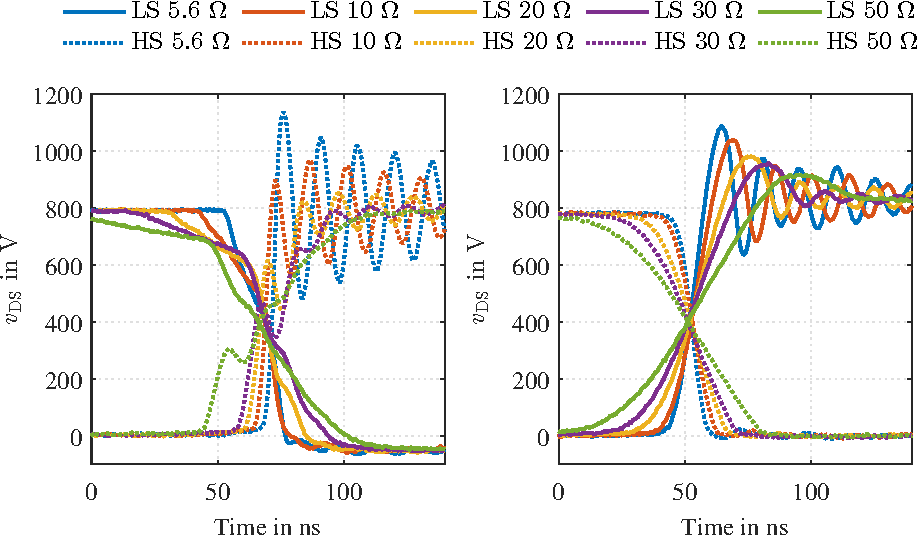
\includegraphics[scale = 1]{figures/7_MeasurementResults/MR_Rg/MR_Rg_Voltage_TD.pdf}
		\subcaption{Time-domain voltage measurement results.}
		\label{fig:MR_Rg_Sweep_Voltage_TD}
	\end{subfigure} 
    
	\vspace{0.5cm}	
	
    \begin{subfigure}[t]{\textwidth}
		\centering
		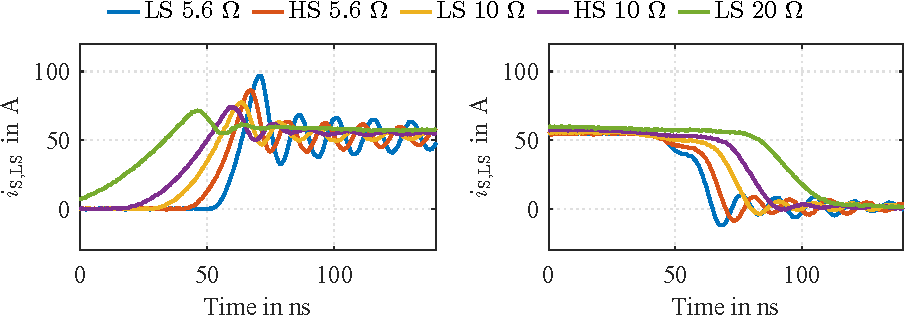
\includegraphics[scale = 1]{figures/7_MeasurementResults/MR_Rg/MR_Rg_Current_TD.pdf}
		\subcaption{Time-domain current measurement results.}
		\label{fig:MR_Rg_Sweep_Current_TD}
	\end{subfigure}
	\caption{Time-domain results of the gate-resistance sweep.}
	\label{fig:MR_Rg_Sweep_TD}
\end{figure}

The structure of the presented measurement results is the same for all external parameters: First, the time-domain voltage and current waveforms are shown, followed by the frequency-domain spectra.
Here, the solid lines are the low-side device, which is for all measurements the active device, and the dashed lines are the high-side device, which is for all measurements the passive device.
Then, the EM emissions are plotted against the switching losses to illustrate the trade-off between these two quantities.
Finally, the EM emissions are separated for turn-on and turn-off to highlight the differences in the emission behavior of these two switching events.

The time domain results of the gate-resistance, shown in Fig.~\ref{fig:MR_Rg_Sweep_TD}, show the expected and well-known trend.
By increasing the gate resistance, from \SI{5.6}{\Omega} to \SI{50}{\Omega}, the switching speed is slowed down by a factor of approximately 10.
This is only slightly shifted due to the internal gate-resistance of the MOSFET of \SI{3.5}{\Omega}, taken from the device datasheet, which adds to the total gate resistance.
Next to the reduced switching speed, the overvoltage and the excited main resonance of the commutaion-loop inductance and the output capacitance of the turned-off device are also reduced, which is a direct consequence of the reduced excitation through the switching transient.

\begin{figure}[ht]
	\centering
	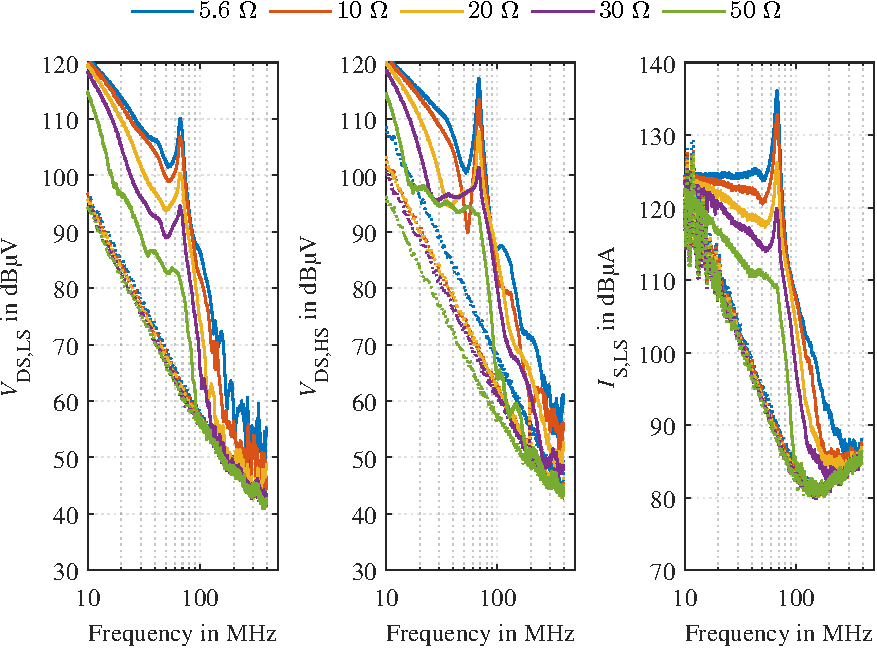
\includegraphics[scale = 1]{figures/7_MeasurementResults/MR_Rg/MR_Rg_FD.pdf}
	\caption{Frequency-domain measurement results of gate resistance sweep.}\label{fig:MR_Rg_Sweep_FD}
\end{figure}

The influence of the gate resistance on the emission spectrum is shown in \fref{fig:MR_Rg_Sweep_FD}, separated for the active and passive device and the commutation current.
Due to the reduced switching speed the entire spectrum is shifted towards lower frequencies, which is a direct consequence of the reduced slew rate of the switching transient.
Additionally, due to that the switching transient is slowed down, the amplitude of the excited main resonance is also reduced up to the point of being no longer clearly visible for \SI{50}{\Omega}.

To quantify the influence of the gate resistance on the EM emissions the spectral average FOM is used, which describes the average emissions for a given frequency range from \SI{30}{\mega\hertz} to \SI{200}{\giga\hertz}.
Here, caution must be taken, because for the highest gate resistance measurements, in the active device, the signal is so low that it still falls below the noise floor more early.
Hence, the average FOM provides an error, it shows a higher value, and thereby less sensitivity for the higher gate resistances.
This effect is a direct consequence of the fundamental measurement noise floor discussed in Section~\ref{sec:MeasurementLimitation}, and it must be kept in mind whenever the average FOM is compared between measurements with strongly differing emission levels, as is the case here for the lowest and the highest gate resistance.

\begin{figure}[ht]
	\centering
	\begin{subfigure}[t]{\textwidth}
		\centering
		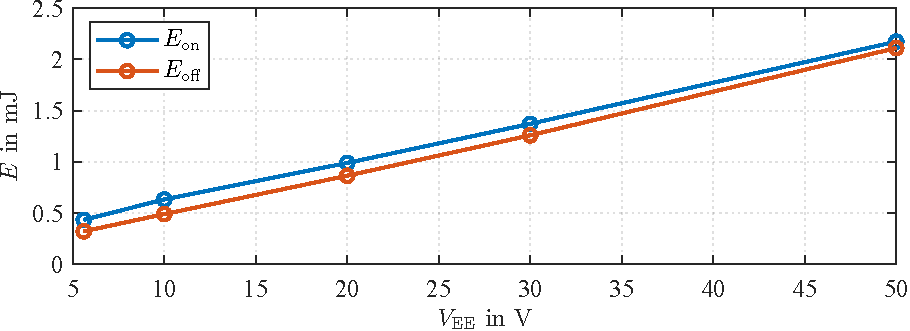
\includegraphics[scale = 1]{figures/7_MeasurementResults/MR_Rg/MR_Rg_Losses.pdf}
		\subcaption{Influence of gate resistance and switching losses on the EM emissions.}
		\label{fig:MR_Rg_EmissionOverLosses}
	\end{subfigure} 

	\vspace{0.5cm}
	
    \begin{subfigure}[t]{\textwidth}
		\centering
		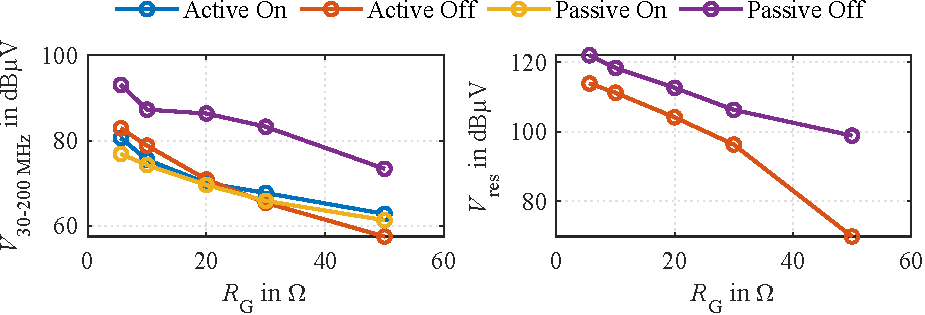
\includegraphics[scale = 1]{figures/7_MeasurementResults/MR_Rg/MR_Rg_Emission.pdf}
		\subcaption{EM emissions separated for turn-on and turn-off.}
		\label{fig:MR_Rg_Emission}
	\end{subfigure}
	\caption{Gate-resistance-dependent emission and loss analysis.}
\end{figure}

The influence of the gate resistance on the switching losses and the EM emissions is shown in \fref{fig:MR_Rg_EmissionOverLosses} and \fref{fig:MR_Rg_Emission}, where the average FOM is plotted against the gate resistance.
Here, the snap-and-mirror function is used to separate the influence of the gate resistance onto the four switching transients, as described in Section~\ref{subsec:SpectralSeparation}.
The analysis shows, next to the spectral average the resonance peak value of the main resonance.
Since the gate resistance has the same impact on all switching transients, the spectrum shows the same trend for all events, only offsetted by the general emission level of the switching event.
When assumed linearly, an influence of \SI{-0.5}{db/\Omega} can be derived for the gate resistance on the average FOM, which is a significant influence, especially when compared to the other external parameters discussed in this section.
For the converter designer, this sensitivity means that, within the limits set by the acceptable switching losses, tuning the gate resistance remains the single most effective lever among the four parameters discussed in this section for trading off EM emissions against switching speed, whereas the remaining parameters, discussed next, offer comparatively smaller but often loss-free means of fine-tuning the emission spectrum.

\FloatBarrier

\subsection{Negative Gate-Driver Bias}

Besides the gate resistance, the negative gate-driver bias \mi{V}{EE} provides a second, independent means to shape the switching transients.
Increasing the magnitude of the negative bias raises the negative overdrive voltage applied to the gate, thereby increasing the driving voltage across the gate loop during turn-off and, consequently, the achievable turn-off speed.
At the same time, a larger negative bias widens the voltage span across which the gate-loop inductance must be charged when the device is switched back on, from \mi{V}{EE} up to the threshold voltage, which prolongs the charging time of the gate loop and thereby delays the onset of the subsequent turn-on transient.
The negative gate-driver bias further affects the freewheeling body diode: as the gate voltage is driven closer to zero, less bipolar charge is stored in the intrinsic body diode, because a less negative bias increasingly allows unipolar channel conduction to contribute to the freewheeling current instead of the diode alone.
The negative gate-driver bias is therefore expected to influence the turn-off- and turn-on-related emissions, as well as the reverse-recovery-related emissions of the freewheeling diode.

\begin{figure}[ht]
	\centering
	\begin{subfigure}[t]{\textwidth}
		\centering
		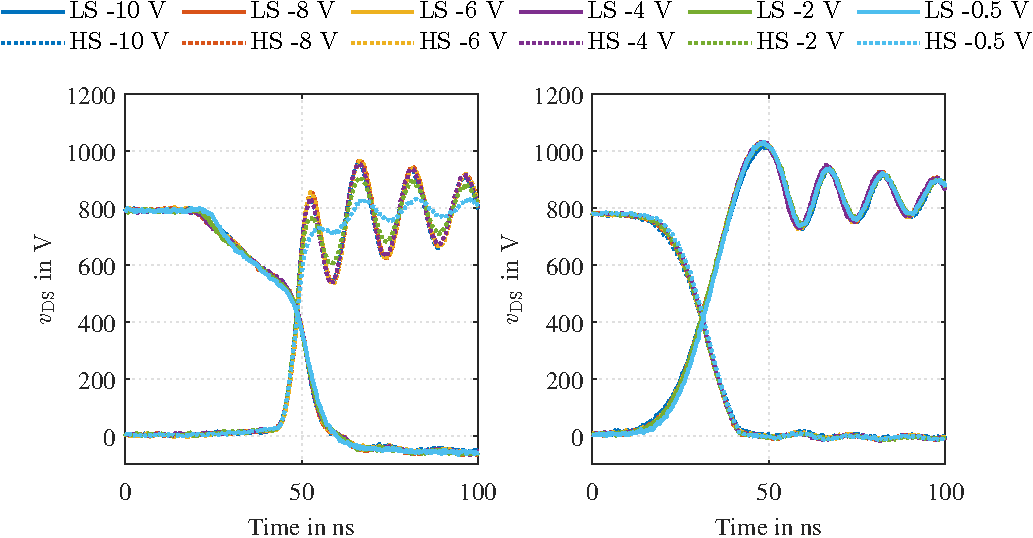
\includegraphics[scale = 1]{figures/7_MeasurementResults/MR_Vee_constE/MR_Vee_constE_Voltage_TD.pdf}
		\subcaption{Time-domain voltage measurement results.}
		\label{fig:MR_Vee_constE_Sweep_Voltage_TD}
	\end{subfigure} 
    
	\vspace{0.5cm}

    \begin{subfigure}[t]{\textwidth}
		\centering
		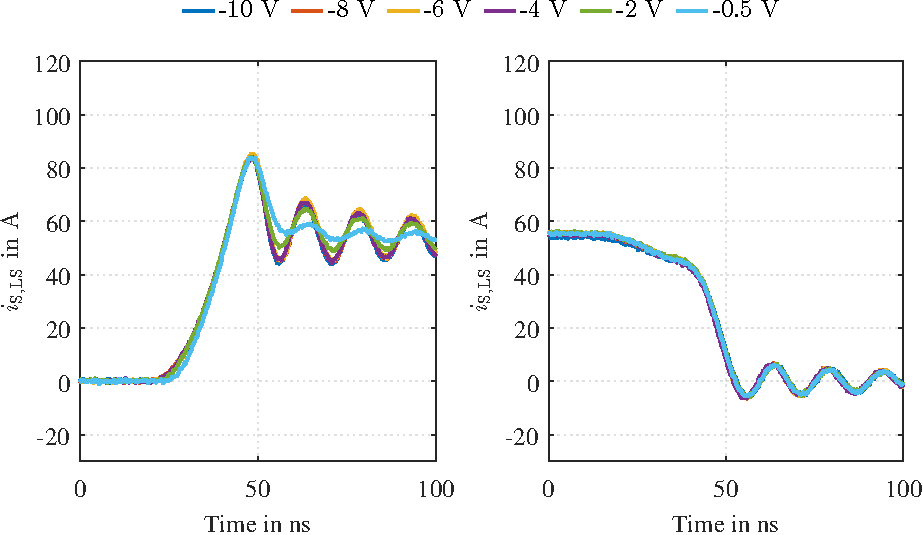
\includegraphics[scale = 1]{figures/7_MeasurementResults/MR_Vee_constE/MR_Vee_constE_Current_TD.pdf}
		\subcaption{Time-domain current measurement results.}
		\label{fig:MR_Vee_constE_Sweep_Current_TD}
	\end{subfigure}
	\caption{Time-domain results of the negative gate-driver bias sweep.}
	\label{fig:MR_Vee_constE_Sweep_TD}
\end{figure}

Fig.~\ref{fig:MR_Vee_constE_Sweep_TD} shows the time-domain results of the negative-gate-driver-bias sweep, covering the range from \SI{-10}{V} to \SI{-0.5}{V}.
Throughout this sweep, the gate resistance is co-adjusted to keep the switching losses constant; as a consequence, the active-off transient, whose speed is governed exclusively by this compensated gate resistance, remains unaffected by the change in bias.
In contrast, a clear influence is observed for the active-on and passive-off transients: between \SI{-10}{V} and \SI{-4}{V} this influence remains minor, whereas for \SI{-2}{V} and \SI{-0.5}{V} the passive switch increasingly loses its resonant ringing behavior.
This trend is consistent with the reduced bipolar charge in the freewheeling diode as the gate bias becomes less negative.


\begin{figure}[ht]
	\centering
	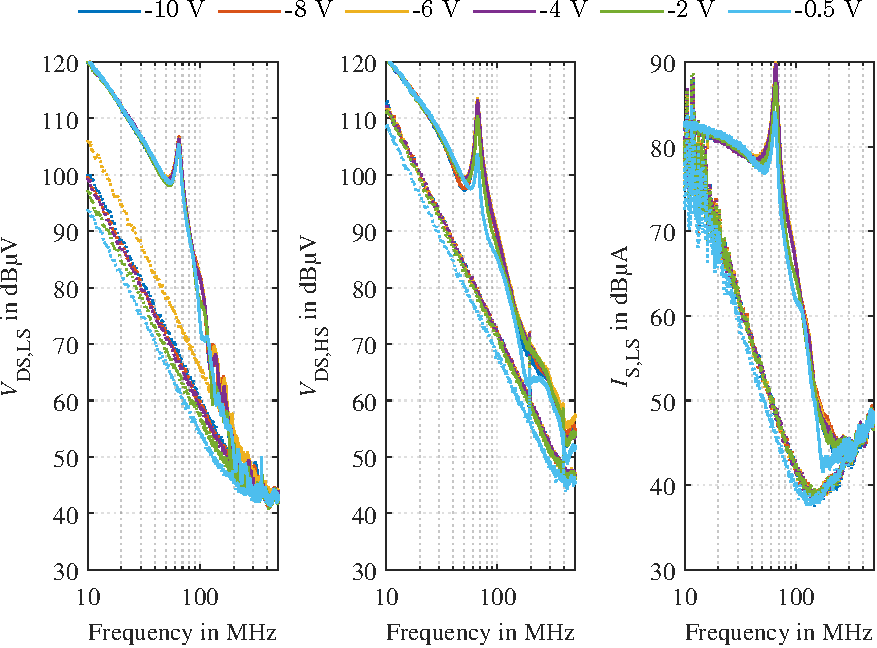
\includegraphics[scale = 1]{figures/7_MeasurementResults/MR_Vee_constE/MR_Vee_constE_FD.pdf}
	\caption{Frequency-domain measurement results of negative gate-driver bias sweep.}\label{fig:MR_Vee_constE_Sweep_FD}
\end{figure}

The corresponding frequency-domain spectra, shown in \fref{fig:MR_Vee_constE_Sweep_FD} and again separated for the active and passive device as well as the commutation current, confirm this trend.
No discernible influence of the negative gate-driver bias is observed in the voltage spectrum between \SI{-10}{V} and \SI{-4}{V}, whereas for \SI{-2}{V} and \SI{-0.5}{V} the main resonance of the passive device is increasingly suppressed and the broadband emissions decrease as a result of the smoother transient.

\begin{figure}[ht]
	\centering
	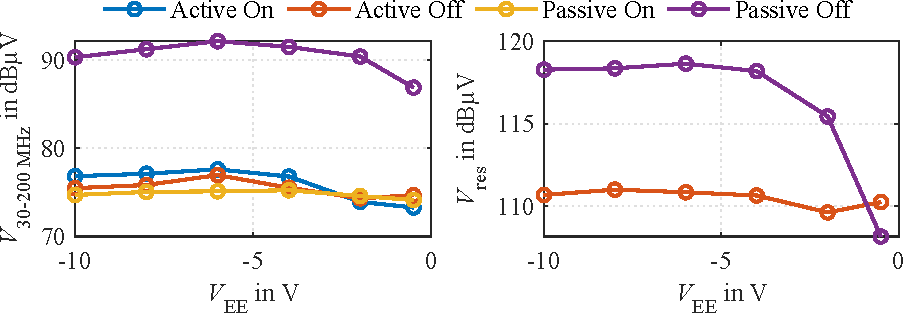
\includegraphics[scale = 1]{figures/7_MeasurementResults/MR_Vee_constE/MR_Vee_constE_Emission.pdf}
	\caption{Influence of the negative gate-driver bias on the EM emission.}\label{fig:MR_Vee_constE_Emission}
\end{figure}

This behavior is quantified in \fref{fig:MR_Vee_constE_Emission}, where the average FOM is plotted against the negative gate-driver bias.
While the active-off and passive-on transients show virtually no dependency, the active-on and passive-off transients exhibit a clear trend: from \SI{-4}{V} to \SI{-0.5}{V} the average FOM decreases by \SI{5}{dB}, a significant influence compared to the other external parameters discussed in this section, and the passive-off resonance peak is damped even more strongly, by \SI{10.5}{dB}.

\FloatBarrier

\subsection{Junction Temperature}

The junction temperature affects several device properties that can be relevant for the switching behavior of the MOSFET, namely the amount of bipolar charge stored in the intrinsic body diode, the threshold voltage \mi{V}{th}, and the internal gate resistance \mi{R}{g,int}.
With increasing temperature, the minority-carrier lifetime in the body diode increases, so that more bipolar charge is stored during freewheeling conduction; upon commutation, this additional charge must be removed as reverse-recovery charge, which is expected to increase the reverse-recovery current peak and to prolong the current tail of the freewheeling device.
The threshold voltage of the SiC MOSFET decreases with increasing temperature, which shifts the gate-source voltage at which channel conduction sets in, thereby speeding up the turn-on and slowing down the turn-off.
The internal gate resistance, in turn, increases with temperature due to the positive temperature coefficient of the polysilicon gate material, which would, on its own, slow down the switching transient.
Since the external gate resistance is co-adjusted in this sweep to keep the switching losses constant, the direct influence of \mi{V}{th} and \mi{R}{g,int} on the switching speed is largely compensated, so that the remaining, temperature-dependent differences in the spectra are expected to be dominated by the reverse-recovery behavior of the freewheeling diode, i.e., the turn-on-related and diode-related emissions.

\begin{figure}[ht]
	\centering
	\begin{subfigure}[t]{\textwidth}
		\centering
		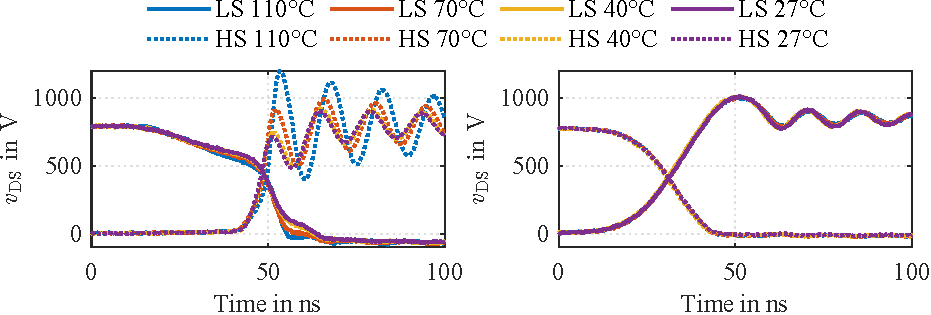
\includegraphics[scale = 1]{figures/7_MeasurementResults/MR_T_constE/MR_T_constE_Voltage_TD.pdf}
		\subcaption{Time-domain voltage measurement results.}
		\label{fig:MR_T_constE_Sweep_Voltage_TD}
	\end{subfigure} 
    
	\vspace{0.5cm}	
	
    \begin{subfigure}[t]{\textwidth}
		\centering
		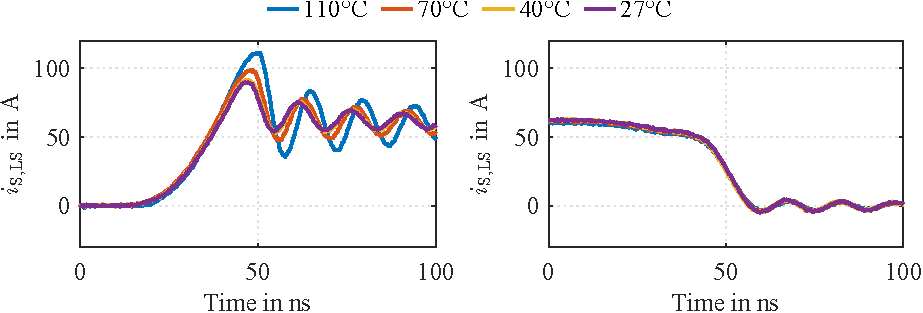
\includegraphics[scale = 1]{figures/7_MeasurementResults/MR_T_constE/MR_T_constE_Current_TD.pdf}
		\subcaption{Time-domain current measurement results.}
		\label{fig:MR_T_constE_Sweep_Current_TD}
	\end{subfigure}
	\caption{Time-domain results of the case-temperature sweep.}
	\label{fig:MR_T_constE_Sweep_TD}
\end{figure}

It must be noted that, in this measurement, the device under test is heated externally from the top of the D2PAK package rather than through the switching losses themselves; consequently, the temperature stated for this sweep, \mi{T}{case}, is a case temperature rather than the junction temperature \mi{T}{j}.
Because the chip is located at the bottom of the package and is thermally connected to the PCB copper acting as a heat sink, so that the actual junction temperature may be somewhat lower than the stated case temperature.
The presented temperature dependency should therefore be interpreted qualitatively as a lower bound on the true sensitivity to the junction temperature.
Additionally, the maximum temperature is limited by the maximum power rating of the used meander structure, the semiconductor chip could be operated at a much higher temperature of atleast \SI{175}{\celsius}.

Fig.~\ref{fig:MR_T_constE_Sweep_TD} shows the time-domain results of the case-temperature sweep, covering the range from \SI{27}{\celsius} to \SI{110}{\celsius}.
The turn-off transient, i.e., the active-off and passive-on switching event, is virtually unaffected by the case temperature: the voltage and current waveforms of all four temperatures overlap almost perfectly.
In contrast, a pronounced temperature dependence is visible for the turn-on transient, i.e., the active-on and passive-off switching event: with increasing case temperature, the reverse-recovery current peak of the freewheeling device increases noticeably, from approximately \SI{89}{\ampere} at \SI{27}{\celsius} to approximately \SI{112}{\ampere} at \SI{110}{\celsius},
and the associated voltage overshoot and ringing of the passive device likewise increase with temperature.
This behavior is consistent with the increased bipolar charge stored in the body diode at elevated temperatures, which must be removed during commutation and thereby increases both the reverse-recovery current and the excitation of the commutation-loop resonance.

\begin{figure}[ht]
	\centering
	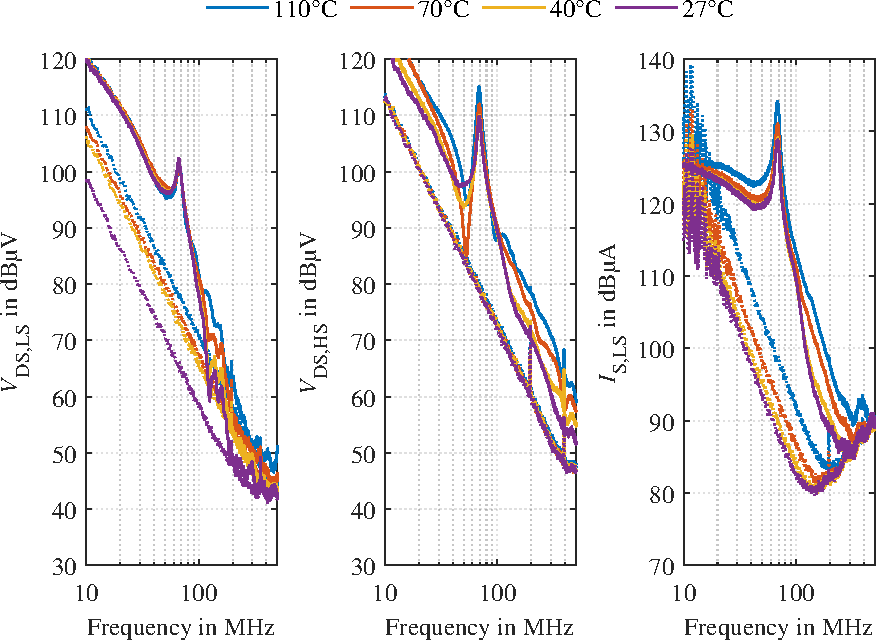
\includegraphics[scale = 0.95]{figures/7_MeasurementResults/MR_T_constE/MR_T_constE_FD.pdf}
	\caption{Frequency-domain measurement results of case-temperature sweep.}\label{fig:MR_T_constE_Sweep_FD}
\end{figure}

The corresponding frequency-domain spectra are shown in \fref{fig:MR_T_constE_Sweep_FD}, separated for the active and passive device and the commutation current.
Across the entire frequency range, the spectra obtained at \SI{27}{\celsius} and \SI{40}{\celsius} lie visibly below those obtained at \SI{70}{\celsius} and \SI{110}{\celsius}, and the resonance peak located around \SI{70}{\mega\hertz}, which is excited by the reverse-recovery-related overshoot, becomes clearly more pronounced as the case temperature increases.
This directly reflects the increasing reverse-recovery charge discussed above: a larger and faster reverse-recovery current excites the commutation-loop resonance more strongly and raises the broadband emission level, particularly for the passive device and the commutation current.

\begin{figure}[ht]
	\centering
	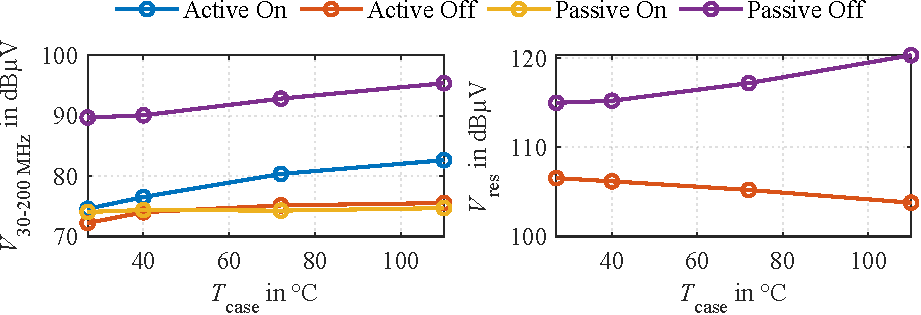
\includegraphics[scale = 1]{figures/7_MeasurementResults/MR_T_constE/MR_T_constE_Emission.pdf}
	\caption{Influence of the temperature on the EM emissions.}
	\label{fig:MR_T_constE_Emission}
\end{figure}

This is quantified in \fref{fig:MR_T_constE_Emission}, where the average FOM and the resonance peak value are plotted against the case temperature, separated for the active and passive device.
The active-off and passive-on transients show virtually no dependency on the case temperature, consistent with the negligible influence observed in the time- and frequency-domain results above.
In contrast, the passive-off transient, i.e., the reverse recovery of the freewheeling diode, shows the strongest temperature dependence among all four transients: the average FOM increases by approximately \SI{6}{\dB} and the resonance peak value increases by approximately \SI{5}{\dB} between \SI{27}{\celsius} and \SI{110}{\celsius}.

The active-on transient, which is only indirectly affected through the current overshoot imposed by the reverse-recovery current of the complementary device, follows the same trend, whereas the resonance peak value of the active-off transient even decreases slightly with increasing temperature.

Considering that this measurement covers only about half of the device's usable temperature range, the junction temperature must nonetheless be regarded as a strong contributor to the EM emissions, an influence that is almost exclusively mediated by the bipolar charge stored in the freewheeling diode.
This finding is particularly significant because the passive-off transient, whose temperature sensitivity is the strongest of all four transients, is already the dominant contributor to the overall EM emissions among all measurements presented in this thesis, even at room temperature.
The junction temperature must therefore be regarded as one of the most important parameters governing the EM emissions of a SiC MOSFET, and it deserves corresponding attention already at the converter design stage by including a temperature margin in the emission budget.

\FloatBarrier

\subsection{Commutation-Loop Inductance}

Unlike the previous three parameters, the commutation-loop inductance \mi{L}{\sigma} is not a free design parameter that is tuned during the development phase to trade off against other requirements, but is always minimized as far as possible. 
It is determined by the physical layout of the power loop, e.g., by the parasitic inductance of the DC-link capacitors, the busbar or PCB traces, and the device packages, and can therefore only be reduced through the layout design.
Together with the output capacitance \mi{C}{oss} of the turned-off device, the commutation-loop inductance forms the resonant tank that is excited by every switching transient.
Increasing \mi{L}{\sigma} raises the characteristic impedance \mi{Z}{0} = \(\sqrt{\mi{L}{\sigma}/\mi{C}{oss}}\) of this tank, which increases the ringing amplitude for a given current excitation, while simultaneously lowering the resonant frequency \mi{f}{res} = $\sfrac{1}{2\pi\sqrt{\mi{L}{\sigma}\mi{C}{oss}}}$.
The commutation-loop inductance is therefore expected to primarily influence the overvoltage and the main resonance of both switching events, shifting it towards lower frequencies and increasing its amplitude, rather than to change the switching speed itself -- considering the speed is set to ensure constant switching losses across the sweep.

\begin{figure}[ht]
	\centering
	\begin{subfigure}[t]{\textwidth}
		\centering
		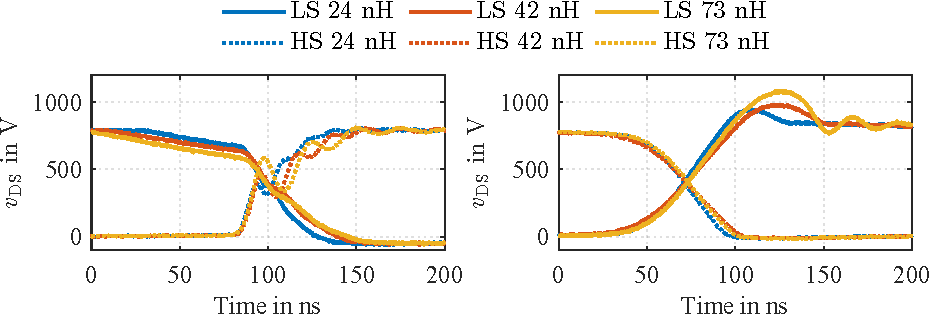
\includegraphics[scale = 1]{figures/7_MeasurementResults/MR_L_constE/MR_L_constE_Voltage_TD.pdf}
		\subcaption{Time-domain voltage measurement results.}
		\label{fig:MR_L_constE_Sweep_Voltage_TD}
	\end{subfigure} 
    
	\vspace{0.5cm}	
	
    \begin{subfigure}[t]{\textwidth}
		\centering
		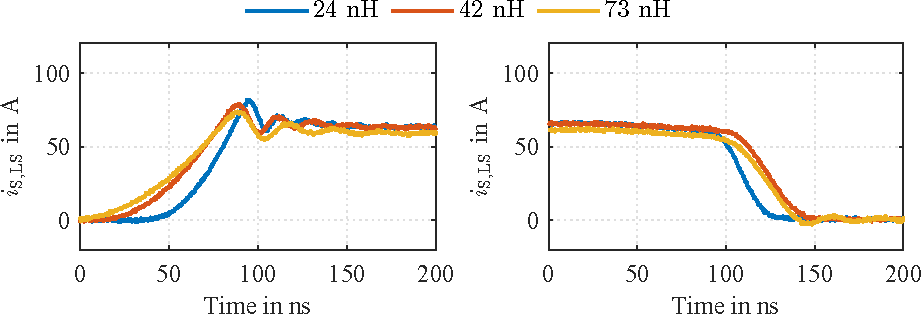
\includegraphics[scale = 1]{figures/7_MeasurementResults/MR_L_constE/MR_L_constE_Current_TD.pdf}
		\subcaption{Time-domain current measurement results.}
		\label{fig:MR_L_constE_Sweep_Current_TD}
	\end{subfigure}
	\caption{Time-domain results of the commutation-loop-inductance sweep.}
	\label{fig:MR_L_constE_Sweep_TD}
\end{figure}

Fig.~\ref{fig:MR_L_constE_Sweep_TD} shows the time-domain results of the commutation-loop-inductance sweep, covering \SI{24}{nH}, \SI{42}{nH}, and \SI{73}{nH}.
Because the gate resistance is co-adjusted for each inductance, the duration of the gate-controlled part of both the turn-on and the turn-off transient remains similar across the sweep.
The ringing that follows each transition, however, changes markedly: with increasing \mi{L}{\sigma}, the peak overvoltage after turn-off grows from \SI{940}{V} at \SI{24}{nH} to \SI{1080}{V} at \SI{73}{nH}, while the ringing frequency visibly decreases, consistent with the larger characteristic impedance and the lower resonant frequency of the \mi{L}{\sigma}-\mi{C}{oss} tank.
A similar, though less pronounced, trend is visible for the ringing excited during turn-on.

\begin{figure}[ht]
	\centering
	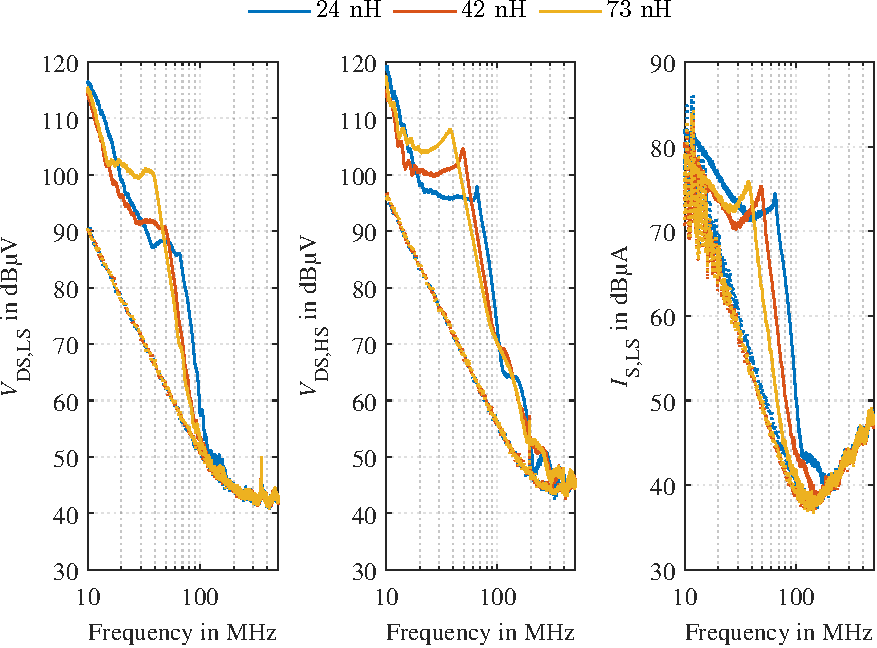
\includegraphics[scale = 1]{figures/7_MeasurementResults/MR_L_constE/MR_L_constE_FD.pdf}
	\caption{Frequency-domain measurement results of the commutation-loop-inductance sweep.}\label{fig:MR_L_constE_Sweep_FD}
\end{figure}

The corresponding frequency-domain spectra, shown in \fref{fig:MR_L_constE_Sweep_FD} and separated for the active and passive device as well as the commutation current, confirm this trend.
Below approximately \SI{10}{\mega\hertz}, the spectra of all three inductances coincide.
Towards higher frequencies, the spectra diverge: for \SI{24}{nH}, the main resonance appears at \SI{66}{\mega\hertz}, whereas for \SI{73}{nH} it shifts down to \SI{37}{\mega\hertz} and reaches a distinctly higher amplitude, in agreement with the lower resonant frequency and the larger characteristic impedance of the commutation loop.

\begin{figure}[ht]
	\centering
	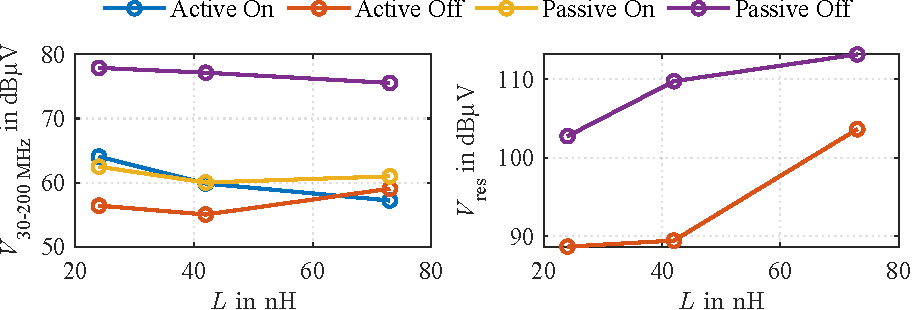
\includegraphics[scale = 1]{figures/7_MeasurementResults/MR_L_constE/MR_L_constE_Emission.pdf}
	\caption{Commutation-loop-inductance-dependent emission and loss analysis.}\label{fig:MR_L_constE_Emission}
\end{figure}

This is quantified in \fref{fig:MR_L_constE_Emission}, where the average FOM and the resonance peak value are plotted against the commutation-loop inductance, separated for the active and passive device and for turn-on and turn-off.
Interestingly, the average FOM does not follow the pronounced increase of the overvoltage observed in the time domain: the passive-off transient, which shows the highest average FOM of all four transients throughout the entire sweep, even decreases slightly, from \SI{78}{dB\micro V} to \SI{75.5}{dB\micro V}, the active-on transient decreases from \SI{64}{dB\micro V} to \SI{57}{dB\micro V}, and the active-off and passive-on transients remain within a narrow band of \SIrange{55}{61}{dB\micro V}.
This apparent contradiction is resolved by the resonance peak value: both the active-off and the passive-off resonance peak increase markedly with the commutation-loop inductance, by approximately \SI{15}{dB} and \SI{9}{dB}, respectively.
The reason is that increasing \mi{L}{\sigma} does not add emission energy, but merely shifts it from higher to lower frequencies, following the falling resonant frequency of the \mi{L}{\sigma}-\mi{C}{oss} tank; such a shift within the averaging window is what the spectral average cannot capture, since it weighs all frequencies within its \SIrange{30}{200}{\mega\hertz} range equally, regardless of where the emissions actually occur.
This highlights an important limitation of a fixed-band average FOM.

Although increasing \mi{L}{\sigma} thereby lowers the emissions at higher frequencies, this seems very unlikely to ever be exploited deliberately as a means to reduce EM emissions, since it comes at the cost of both increased low-frequency emissions and a higher overvoltage.
Since \mi{L}{\sigma} is fixed by the power-stage layout rather than by the gate driver or the device, this influence cannot be corrected during operation; it must therefore be addressed already during the layout design of the commutation loop, for instance by minimizing the enclosed loop area and by placing the DC-link capacitors as close as possible to the switching devices.
%!TeX root = main.tex
%!encoding = UTF-8 Unicode
\section{Influence of MOSFET Parameters}
\label{sec:MR_MOSFET}

This section examines the influence of parameters that are determined by the device engineer during MOSFET design, namely the active chip area and the SiC technology generation.
Both parameters directly affect the device's parasitic capacitances and the resulting switching trajectory, so unlike the external parameters discussed in Section~\ref{sec:MR_External}, they cannot be tuned by the application engineer once a device has been selected.
For each parameter, a comparison is performed while the switching losses are kept constant, so that the differences observed in the frequency-domain spectra can be attributed to the parameter itself rather than to a shift in the switching trajectory.

\subsection{Active Chip Area}


\begin{figure}[ht]
	\centering
	\begin{subfigure}[t]{\textwidth}
		\centering
		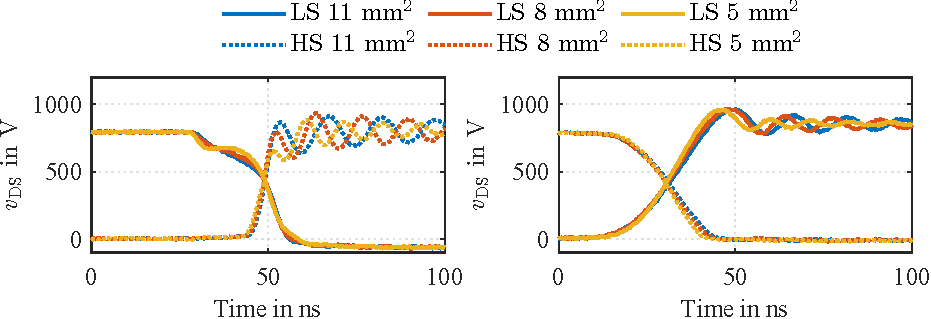
\includegraphics[scale = 1]{figures/7_MeasurementResults/MR_A_constE/MR_A_constE_Voltage_TD.pdf}
		\subcaption{Time-domain voltage measurement results.}
		\label{fig:MR_A_constE_Sweep_Voltage_TD}
	\end{subfigure} 
    
	\vspace{0.5cm}	
	
    \begin{subfigure}[t]{\textwidth}
		\centering
		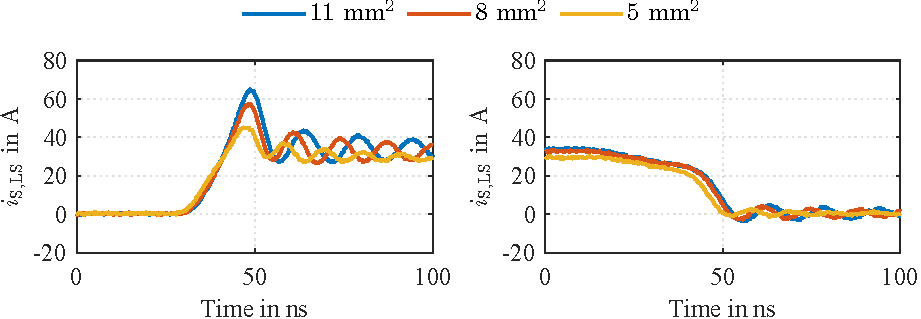
\includegraphics[scale = 1]{figures/7_MeasurementResults/MR_A_constE/MR_A_constE_Current_TD.pdf}
		\subcaption{Time-domain current measurement results.}
		\label{fig:MR_A_constE_Sweep_Current_TD}
	\end{subfigure}
	\caption{Time-domain results of the negative gate-driver bias sweep.}
\end{figure}

\begin{figure}[ht]
	\centering
	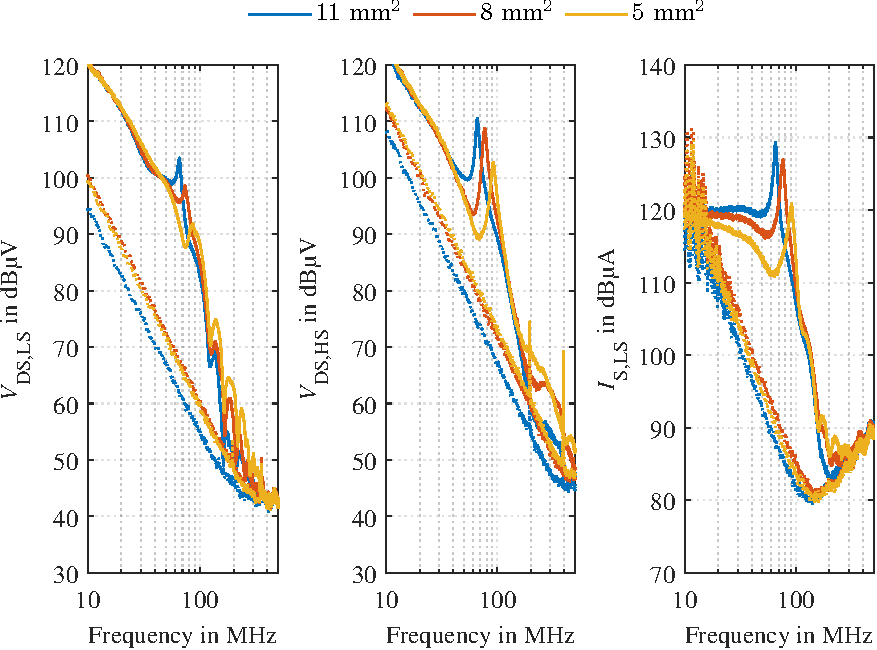
\includegraphics[scale = 1]{figures/7_MeasurementResults/MR_A_constE/MR_A_constE_FD.pdf}
	\caption{Frequency-domain measurement results of negative gate-driver bias sweep.}\label{fig:MR_A_constE_Sweep_FD}
\end{figure}


\begin{figure}[ht]
	\centering
	\begin{subfigure}[t]{\textwidth}
		\centering
		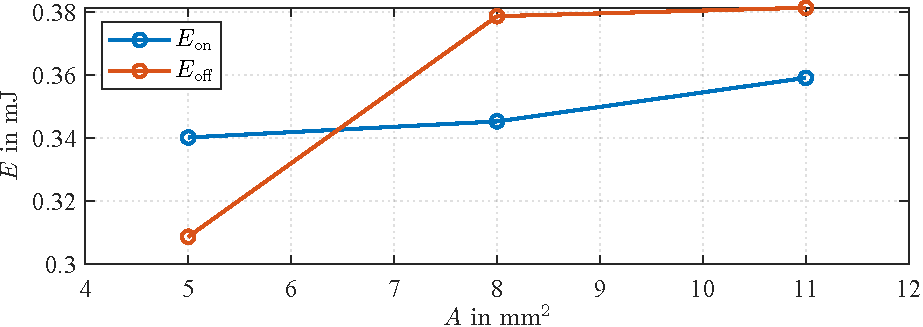
\includegraphics[scale = 1]{figures/7_MeasurementResults/MR_A_constE/MR_A_constE_Losses.pdf}
		\subcaption{Influence of negative gate-driver bias and switching losses on the EM emissions.}
		\label{fig:MR_A_constE_EmissionOverLosses}
	\end{subfigure} 

	\vspace{0.5cm}
	
    \begin{subfigure}[t]{\textwidth}
		\centering
		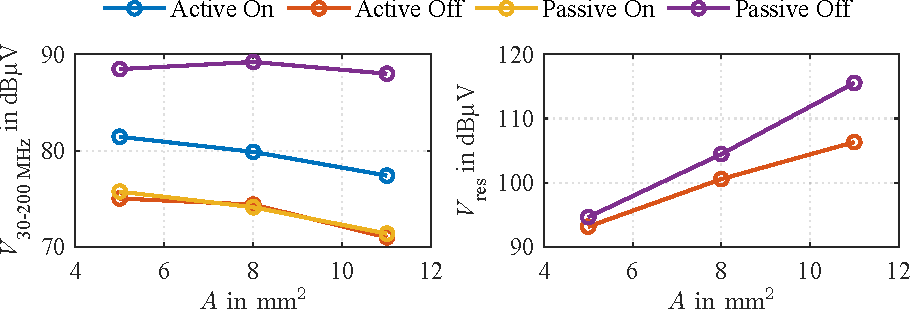
\includegraphics[scale = 1]{figures/7_MeasurementResults/MR_A_constE/MR_A_constE_Emission.pdf}
		\subcaption{EM emissions separated for turn-on and turn-off.}
		\label{fig:MR_A_constE_Emission}
	\end{subfigure}
	\caption{Negative gate-driver-bias-dependent emission and loss analysis.}
\end{figure}



\subsection{SiC Technology Generation}

\begin{figure}[ht]
	\centering
	\begin{subfigure}[t]{\textwidth}
		\centering
		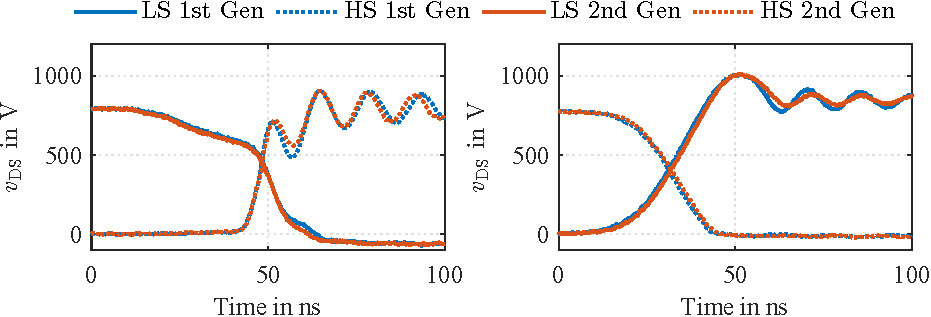
\includegraphics[scale = 1]{figures/7_MeasurementResults/MR_Gen_constE/MR_Gen_constE_Voltage_TD.pdf}
		\subcaption{Time-domain voltage measurement results.}
		\label{fig:MR_Gen_constE_Sweep_Voltage_TD}
	\end{subfigure} 
    
	\vspace{0.5cm}	
	
    \begin{subfigure}[t]{\textwidth}
		\centering
		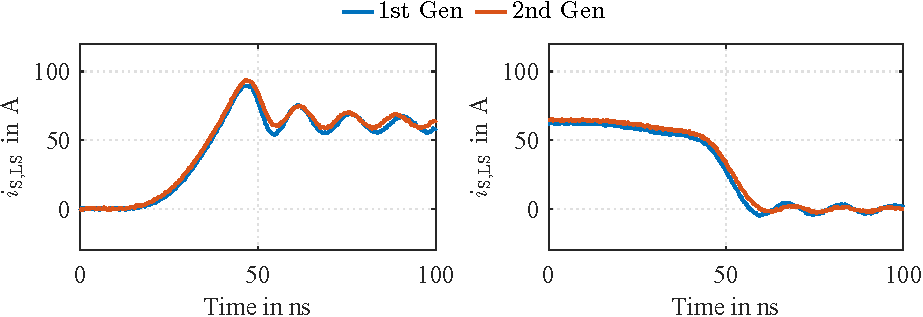
\includegraphics[scale = 1]{figures/7_MeasurementResults/MR_Gen_constE/MR_Gen_constE_Current_TD.pdf}
		\subcaption{Time-domain current measurement results.}
		\label{fig:MR_Gen_constE_Sweep_Current_TD}
	\end{subfigure}
	\caption{Time-domain results of the negative gate-driver bias sweep.}
\end{figure}

\begin{figure}[ht]
	\centering
	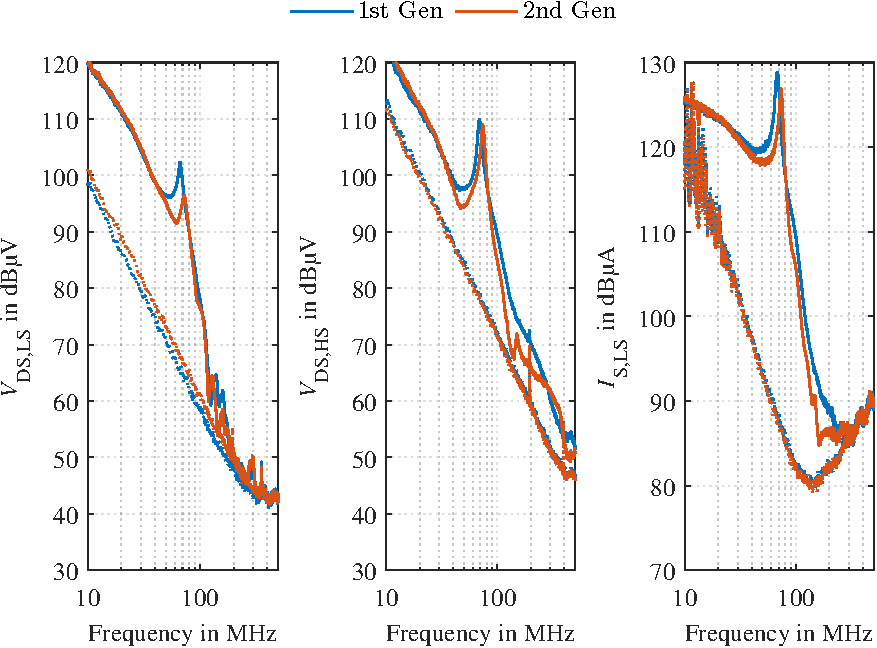
\includegraphics[scale = 1]{figures/7_MeasurementResults/MR_Gen_constE/MR_Gen_constE_FD.pdf}
	\caption{Frequency-domain measurement results of negative gate-driver bias sweep.}\label{fig:MR_Gen_constE_Sweep_FD}
\end{figure}


\begin{figure}[ht]
	\centering
	\begin{subfigure}[t]{\textwidth}
		\centering
		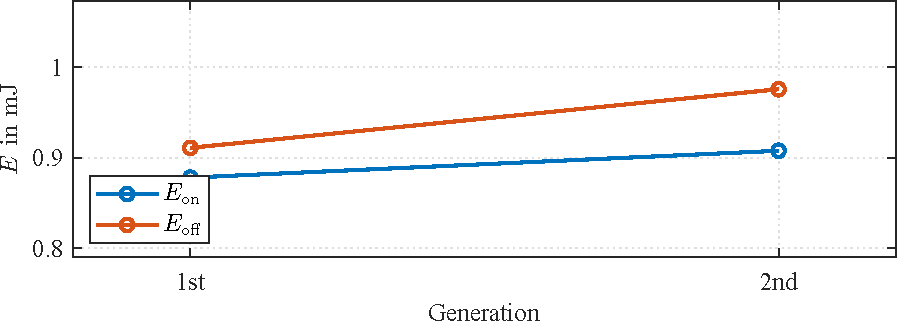
\includegraphics[scale = 1]{figures/7_MeasurementResults/MR_Gen_constE/MR_Gen_constE_Losses.pdf}
		\subcaption{Influence of negative gate-driver bias and switching losses on the EM emissions.}
		\label{fig:MR_Gen_constE_EmissionOverLosses}
	\end{subfigure} 

	\vspace{0.5cm}
	
    \begin{subfigure}[t]{\textwidth}
		\centering
		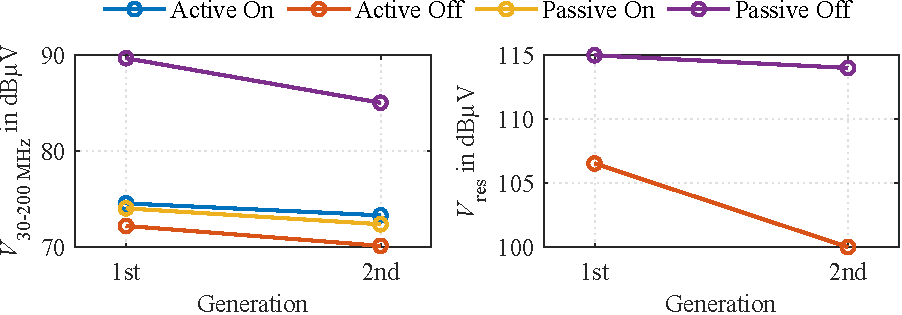
\includegraphics[scale = 1]{figures/7_MeasurementResults/MR_Gen_constE/MR_Gen_constE_Emission.pdf}
		\subcaption{EM emissions separated for turn-on and turn-off.}
		\label{fig:MR_Gen_constE_Emission}
	\end{subfigure}
	\caption{Negative gate-driver-bias-dependent emission and loss analysis.}
\end{figure}



\subsection*{Benchmarking of SiC MOSFET Manufacturers}

Beyond device-parameter studies, the proposed measurement environment also enables benchmarking of semiconductor technologies.
To demonstrate this capability and to establish EM emission as a design dimension in addition to classical trade-offs, a comparative market analysis of four SiC MOSFET devices from different manufacturers is presented.

All evaluated devices are \SI{1200}{V} SiC MOSFETs in D2PAK packages with a current rating of $\SI{60}{A}\pm\SI{5}{A}$ and are operated at $\mi{V}{DC}~=~\SI{800}{V}$ and $\mi{I}{L}~=~\SI{60}{A}$ at room temperature.

\begin{figure}[h]
	\centering
	% \includegraphics[scale = 1]{MeasurementResults/MR_MarketOverview}
	\input{7_MeasurementResults/MR_MarketOverview.tex}
	\caption{Comparative analysis of EM noise emission performance for SiC MOSFETs from different manufacturers.}\label{fig:MR_CompetitorAnalysis}
\end{figure}

Because a fair comparison at a single operating point is difficult, a gate-resistance sweep of $\mbox{\mi{R}{G,ext} = [1, 5, 10, 20, 30, 50]~\si{\ohm}}$ is performed, with an overvoltage limit of \SI{1200}{V} as the stopping criterion.
% Therefore, a gate-resistance sweep of $\mi{R}{G} = [1, 5, 10, 20, 30, 50]~\si{\ohm}$ is performed, with an overvoltage limit of \SI{1200}{V} as the stopping criterion.
The gate resistance sweep visualizes the trade-off between switching losses and EM noise emission for a given technology.
Hence, for each operating point, the switching loss energy \mi{E}{sw,tot} is calculated together with the average spectral emission of the active and passive switch voltages~\cite{kragl_impact_2024}:

% \begin{equation}
% 	\bar{V}_\mathrm{20-300MHz}^\mathrm{LS,HS} = 20 \log_{10}\left(\frac{\Delta\mi{f}{bin}\sum\limits_{\SI{20}{MHz}}^{\SI{300}{MHz}} \left(\mi{V}{DS,LS}[n] + \mi{V}{DS,HS}[n]\right)}{2\cdot(\SI{300}{MHz} - \SI{20}{MHz})\cdot\SI{1}{\micro V}}\right) 
% \end{equation}

\begin{equation}
	\bar{V}_\mathrm{20-300MHz}^\mathrm{LS,HS} = 20 \log_{10}\frac{\Delta\mi{f}{bin}\sum\limits_{\SI{20}{MHz}}^{\SI{300}{MHz}} \left(\mi{V}{DS,LS}[n] + \mi{V}{DS,HS}[n]\right)}{2\cdot(\SI{300}{MHz} - \SI{20}{MHz})\cdot\SI{1}{\micro V}}
\end{equation}


The resulting comparison, plotted in \fref{fig:MR_CompetitorAnalysis}, shows a clear and expected trend of increasing EM noise emission with decreasing switching energy.
However, the results also show that different devices emit up to \SI{7}{dB} higher average noise levels, with significantly higher differences at specific frequencies.
This establishes EM noise as a design dimension alongside classical trade-offs, and demonstrates the capability of the introduced measurement environment.


%!TeX root = main.tex
%!encoding = UTF-8 Unicode
\section{Summary of Measurement Studies}
\label{sec:MR_Summary}

\begin{table}[ht]
	\caption{Summary of the impact of different parameters on the active-off and passive-off measurement results.}
	\label{tab:SummaryMRStudies}
	\centering
	\setlength{\tabcolsep}{18pt}
	\begin{tabular}{@{}lccl@{}}
		\toprule
		\textbf{Parameter} & \textbf{Active Off} & \textbf{Passive Off} & \textbf{Condition} \\
		\midrule
		\multirow{2}{*}{Gate drive} & -0.56 dB/$\Omega$ & -0.39 dB/$\Omega$ & \mi{R}{G} sweep \\
		                            & -14.53 dB/mJ & -9.88 dB/mJ & \mi{R}{G} sweep \\
		\midrule
		\multirow{3}{*}{Chip Size $A$} & -0.92 dB/mm & -0.59 dB/mm  & Const. \mi{R}{G} \\
		                    & -0.92 dB/mm  & -0.38 dB/mm  & Const. OV \\
		                    & -0.67 dB/mm  & -0.08 dB/mm  & Const. \mi{E}{sw} \\
		\midrule
		\multirow{3}{*}{\shortstack[l]{Neg. Driver Supply\\\mi{V}{ee,driver}}} & -0.67 dB/V & -0.47 dB/V & Const. \mi{R}{G} \\
		                                      & +0.08 dB/V & +0.23 dB/V & Const. OV \\
		                                      & -0.15 dB/V & -0.29 dB/V & Const. \mi{E}{sw} \\
		\midrule
		\multirow{3}{*}{Temperature $T$} & 0.005 dB/K & 0.064 dB/K & Const. \mi{R}{G} \\
		                    & 0.003 dB/K & 0.013 dB/K & Const. OV \\
		                    & 0.035 dB/K & 0.071 dB/K & Const. \mi{E}{sw} \\
		\midrule
		\multirow{3}{*}{\shortstack[l]{Commutaion-Loop\\ Inductance \mi{L}{\sigma}}} & 0.09 dB/nH & 0.01 dB/nH & Const. \mi{R}{G} \\
		                              & -0.41 dB/nH & -0.12 dB/nH & Const. OV \\
		                              & 0.06 dB/nH & -0.05 dB/nH & Const. \mi{E}{sw} \\
		\midrule
		\multirow{3}{*}{Bosch Generation} & +3 dB/Gen & -4.5 dB/Gen & Const. \mi{R}{G} \\
		                                  & -3.5 dB/Gen & -2.9 dB/Gen & Const. OV \\
		                                  & -2.1 dB/Gen & -4.6 dB/Gen & Const. \mi{E}{sw} \\
		\bottomrule
	\end{tabular}
\end{table}




